\documentclass{beamer}
\usepackage[skins,minted,breakable]{tcolorbox}
\usepackage[spanish]{babel}
\usepackage{subcaption}
\usetikzlibrary{matrix,backgrounds}
\usepackage{multirow}
\usepackage{hyperref}
\usepackage{multicol}
\usepackage{adjustbox}
\usepackage{soul}
\usepackage{listings}
\usepackage{graphicx}% http://ctan.org/pkg/graphicx
\usepackage{booktabs}% http://ctan.org/pkg/booktabs
\usepackage{tikz}
\usetikzlibrary{shapes.geometric, arrows, chains, calc,positioning,fit,decorations.pathreplacing}
\usepackage[framemethod=tikz]{mdframed}
\definecolor{light-gray}{gray}{0.95}

\lstset{
  basicstyle=\footnotesize,
}
\lstset{columns=fullflexible,basicstyle=\ttfamily}
\surroundwithmdframed[
  hidealllines=true,
  backgroundcolor=light-gray,
  innerleftmargin=0pt,
  innertopmargin=0pt,
  innerbottommargin=0pt]{lstlisting}

\graphicspath{ {../img/}}
\selectlanguage{spanish}
\usepackage[utf8]{inputenc}
\usetheme{PaloAlto}
\setbeamerfont{section in sidebar}{size=\fontsize{2}{4}\selectfont}
\setbeamerfont{subsection in sidebar}{size=\fontsize{2}{3}\selectfont}
\setbeamerfont{subsubsection in sidebar}{size=\fontsize{2}{2}\selectfont}

\setbeamerfont{section in toc}{size=\footnotesize}
\setbeamerfont{subsection in toc}{size=\scriptsize}
\setbeamerfont{subsubsection in toc}{size=\tiny}

\hypersetup{
    urlcolor=cyan           % color of external links
}

\makeatletter
\def\Opacity{1}
\addtobeamertemplate{headline}{}{%
\begin{tikzpicture}[remember picture,overlay]
\ifnum\theframenumber=1\relax\else\def\Opacity{0.3}\fi
  \node[opacity=\Opacity,anchor=north,inner sep=0pt,outer sep=0pt]
  at ([xshift=0.5\beamer@sidebarwidth]current page.north)
  {
\includegraphics[
    height=\beamer@headheight
    ]{project/title_logo.png}};
\end{tikzpicture}%
}
\makeatother

\title{Servidores Web de Altas Prestaciones}
\date{25 de Mayo de 2020}
\subtitle{Desplegando una granja web en Google Cloud Platform}

\author{Carlos Sánchez Páez}

\makeatletter
  \setbeamertemplate{sidebar \beamer@sidebarside}%{sidebar theme}
  {
    \beamer@tempdim=\beamer@sidebarwidth%
    \advance\beamer@tempdim by -6pt%
    \insertverticalnavigation{\beamer@sidebarwidth}%
    \vfill
    \ifx\beamer@sidebarside\beamer@lefttext%
    \else%
      \usebeamercolor{normal text}%
      \llap{\usebeamertemplate***{navigation symbols}\hskip0.1cm}%
      \vskip2pt%
    \fi%
}%
\makeatother

\subject{Servidores Web de Altas Prestaciones}

% Let's get started
\begin{document}
\AtBeginSection[]
  {
     \begin{frame}<beamer>
     \frametitle{Índice}
     \tableofcontents[currentsection]
     \end{frame}
  }
\AtBeginSubsection[]
{
  \begin{frame}<beamer>{Índice}
    \tableofcontents[currentsection,currentsubsection]
  \end{frame}
}
\AtBeginSubsubsection[]
{
  \begin{frame}<beamer>{Índice}
    \tableofcontents[currentsection,currentsubsection]
  \end{frame}
}
\centering
\begin{frame}
 \titlepage
\end{frame}

\begin{frame}{Índice}
 \tableofcontents
 % You might wish to add the option [pausesections]
\end{frame}

\section{Objetivo del proyecto}

\begin{frame}[fragile]{Objetivo del proyecto}
  Despliegue de una granja web capaz de \textbf{autoescalar}.
\end{frame}

\begin{frame}[fragile]{¿Qué es \textbf{autoescalar}?}
  \begin{figure}[H]
    \centering
    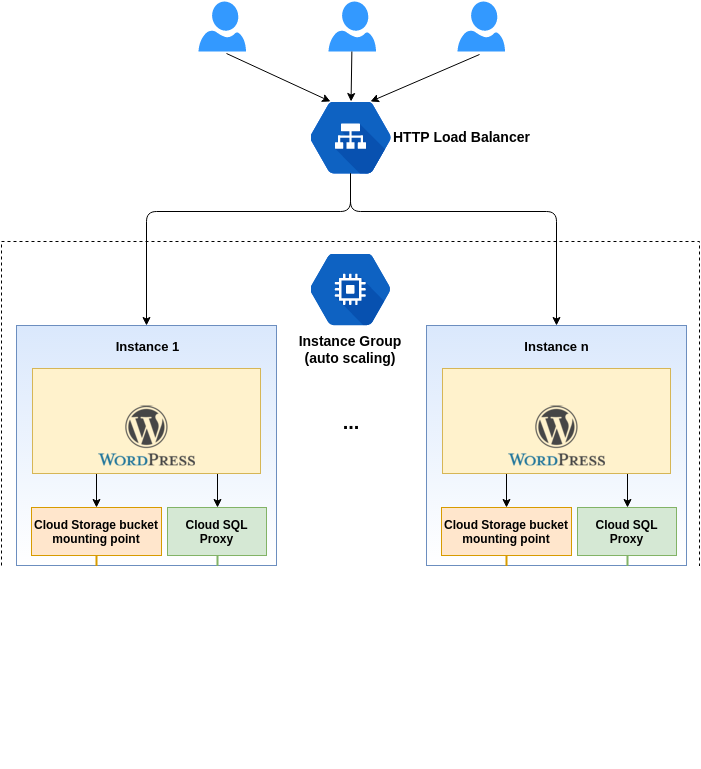
\includegraphics[width =0.8\textwidth]{project/autoscaling.png}
  \end{figure}
\end{frame}

\begin{frame}[fragile]{Arquitectura a desplegar}
  \begin{figure}[H]
    \centering
    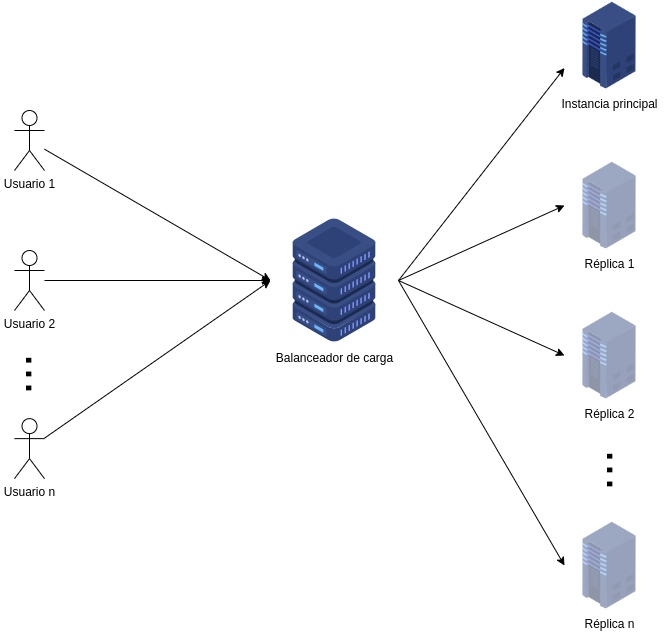
\includegraphics[width =0.7\textwidth]{project/architecture.png}
  \end{figure}
\end{frame}

\section{Google Cloud Platform}

\subsection{Qué es Google Cloud Platform?}

\begin{frame}[fragile]{Qué es Google Cloud Platform?}
  \begin{itemize}[<+->]
    \item Conjunto de recursos de computación que Google usa para sus productos.
    \item Tercera empresa mundial en el mercado de Cloud Computing.
    \item Ofrece IaaS, PaaS y SaaS mediante más de 50 productos.
  \end{itemize}
\end{frame}


\begin{frame}[fragile]{Ventajas de GCP}
  \begin{itemize}[<+->]
    \item Tutoriales interactivos
    \item Panel de control con estadísticas y métricas.
    \item Aplicación para Android e iOS.
    \item Prueba gratuita de 300\$.
    \item Terminal web e interfaz CLI (\emph{gcloud}).
  \end{itemize}
\end{frame}

\subsection{Quién la utiliza?}

\begin{frame}[fragile]{Quién la utiliza?}
\begin{figure}[H]
  \centering
  
\includegraphics[width =\textwidth]{project/logos.png}
\end{figure}
Más de 4 millones de clientes que pagan (Febrero 2018).
\end{frame}

\subsection{Productos de Google Cloud Platform}

\begin{frame}[fragile]{Productos de Google Cloud Platform}
\begin{figure}[H]
  \centering
  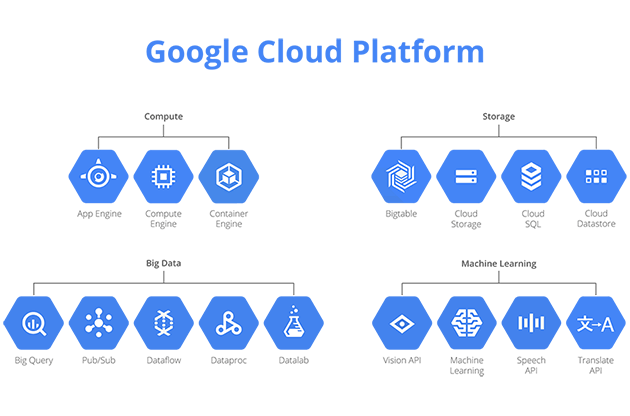
\includegraphics[width =\textwidth]{project/gcp_products.png}
\end{figure}
\end{frame}

\begin{frame}[fragile]{Productos de Google Cloud Platform}
\begin{figure}[H]
  \centering
  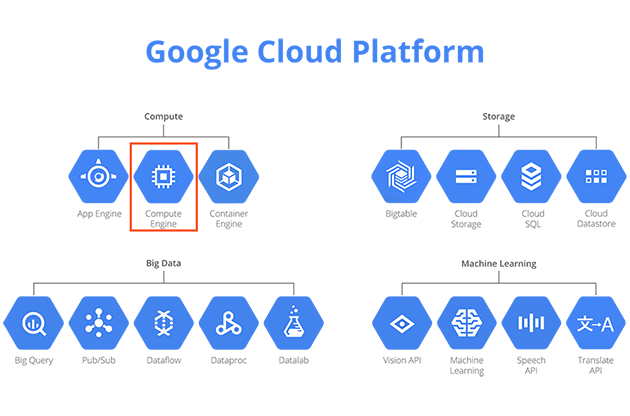
\includegraphics[width =\textwidth]{project/gcp_products_select.png}
\end{figure}
\end{frame}

\section{Despliegue de la granja web}

\subsection{¿Qué necesitamos?}

\begin{frame}[fragile]{¿Qué necesitamos?}
  \begin{itemize}[<+->]
    \item Proyecto en la plataforma
    \item Red para las instancias y el balanceador.
    \begin{itemize}[<+->]
      \item Firewall
    \end{itemize}
    \item Grupo de instancias.
    \begin{itemize}[<+->]
      \item Plantilla para las instancias
    \end{itemize}
    \item Balanceador de carga.
    \begin{itemize}[<+->]
      \item Comprobación de estado
    \end{itemize}
  \end{itemize}
\end{frame}

\subsubsection{Proyecto en la plataforma}

\begin{frame}[fragile]{Creación del proyecto}
  \begin{figure}[H]
		\centering
		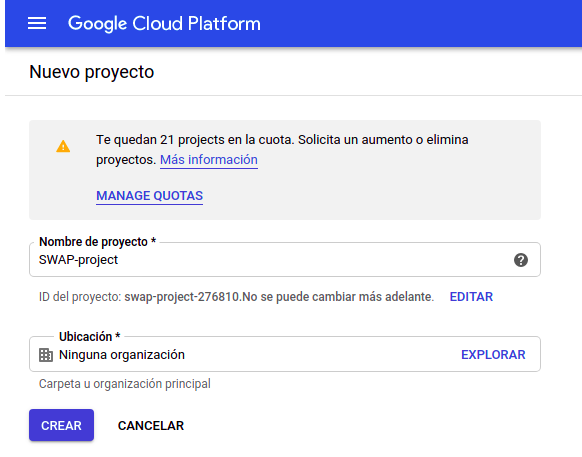
\includegraphics[width=0.5\textwidth]{project/create_project.png}
	\end{figure}
\end{frame}

\subsubsection{Red para las instancias y el balanceador}

\begin{frame}[fragile]{Creación de la red}
  \begin{figure}[H]
		\centering
		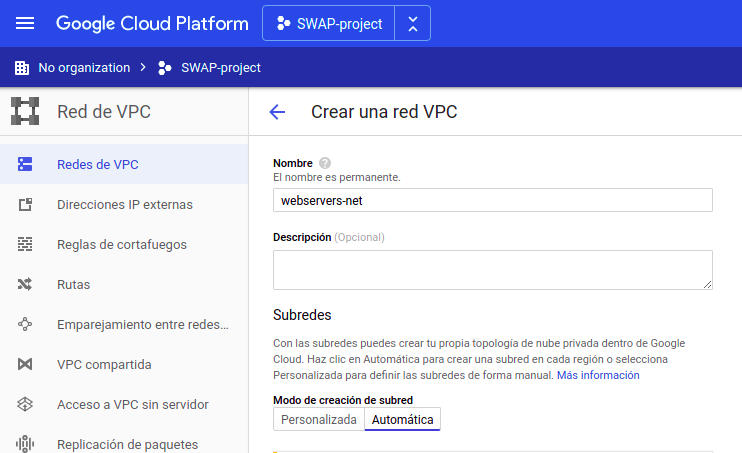
\includegraphics[width=0.5\textwidth]{project/vpc_creation.png}
	\end{figure}
\end{frame}

\begin{frame}[fragile]{Creación de la regla de firewall}
  \begin{figure}[H]
		\centering
		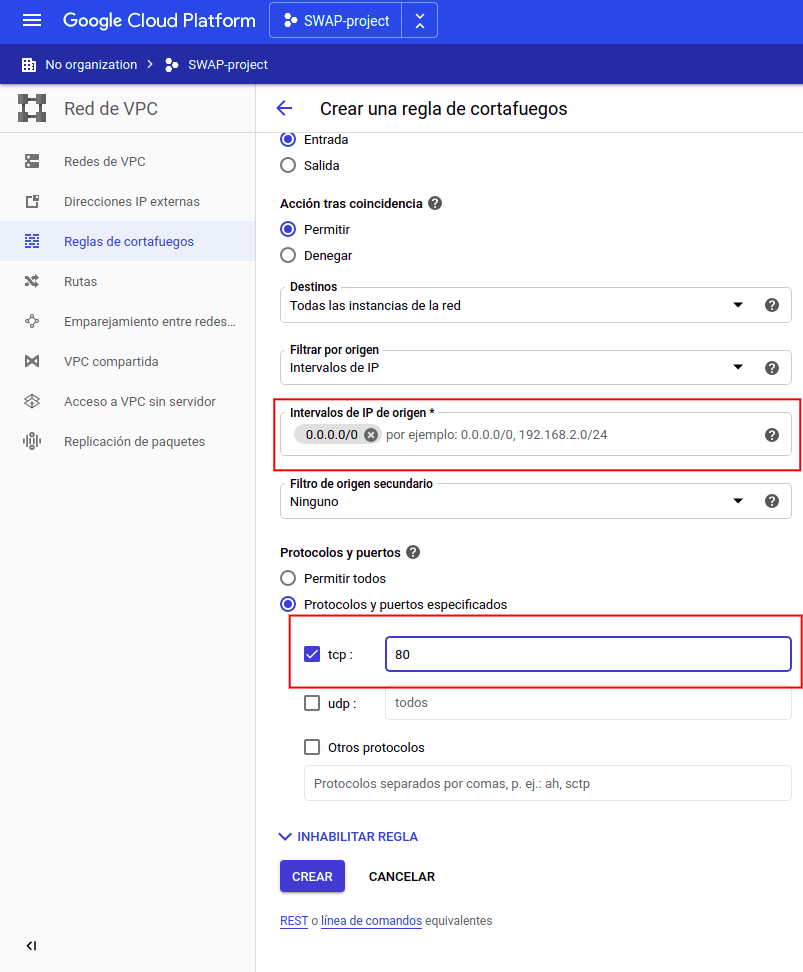
\includegraphics[width=0.5\textwidth]{project/firewall_creation.png}
	\end{figure}
\end{frame}

\subsubsection{Grupo de instancias}


\begin{frame}[fragile]{Creación del grupo de instancias}
  \begin{figure}[H]
		\centering
		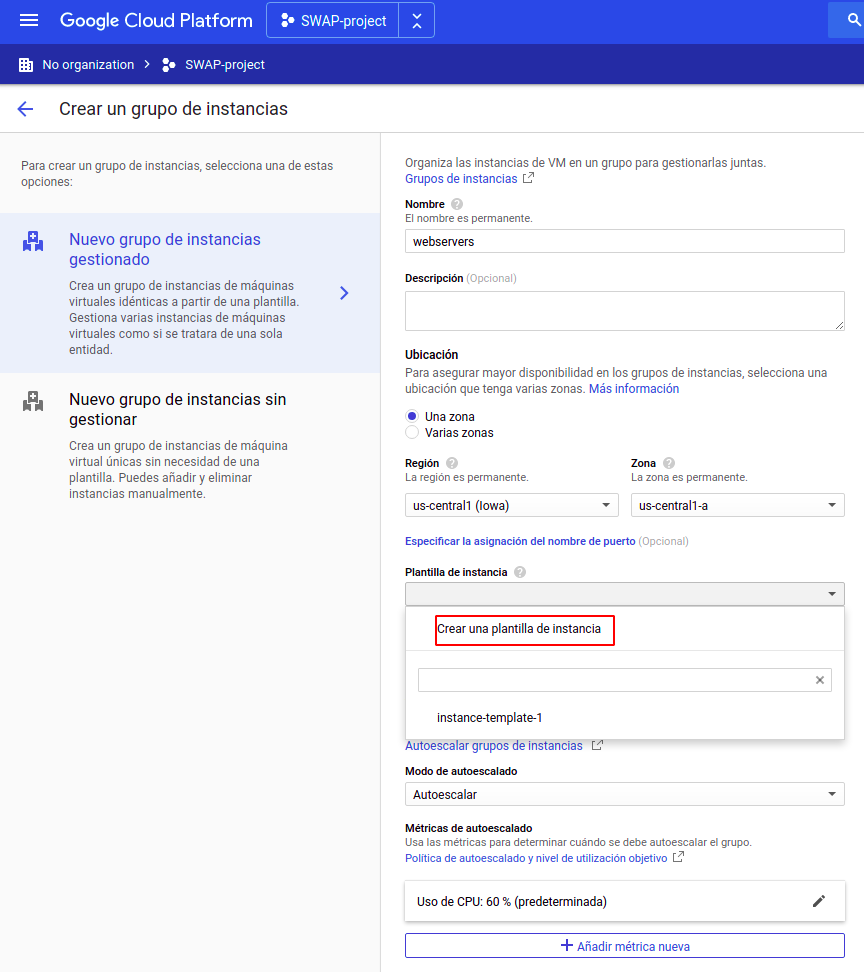
\includegraphics[width=0.5\textwidth]{project/createig.png}
	\end{figure}
\end{frame}

\begin{frame}[fragile]{Creación de la plantilla}
  \begin{figure}[H]
		\centering
		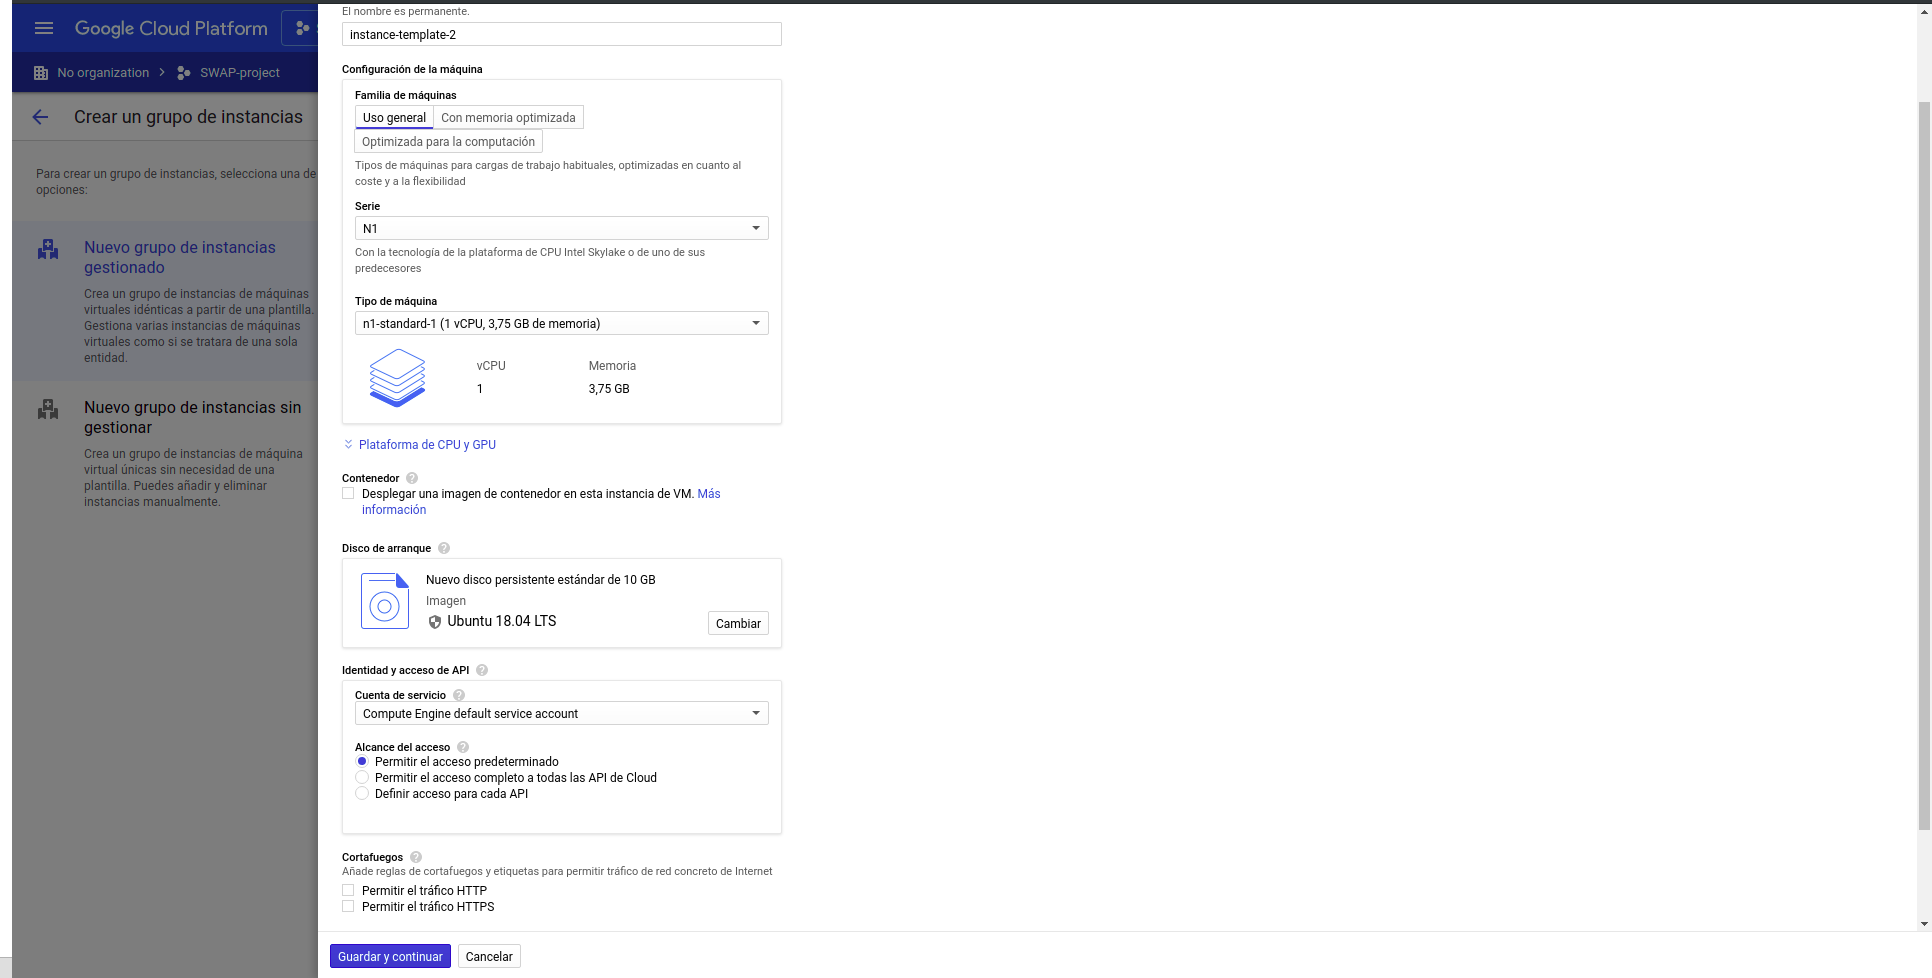
\includegraphics[width=0.45\textwidth]{project/createtemplate.png}
	\end{figure}
\end{frame}

\begin{frame}[fragile]{Instalación del servidor web en las instancias}
  \begin{figure}[H]
		\centering
		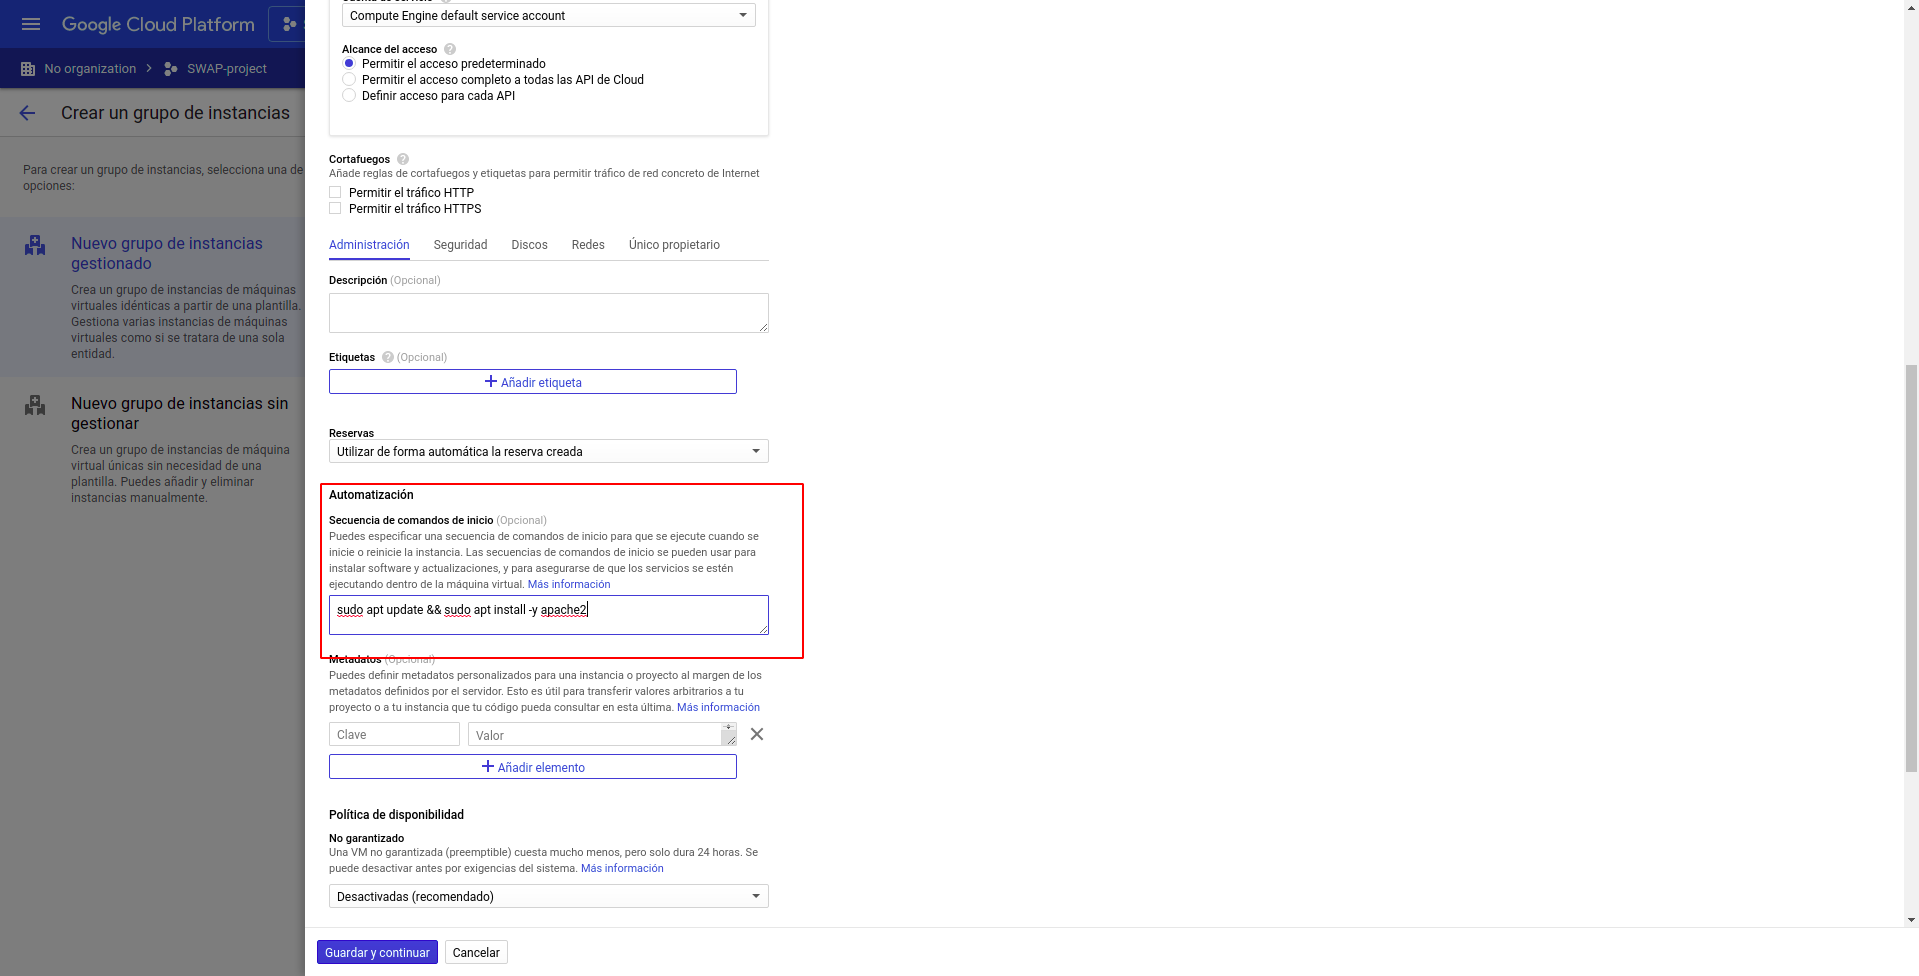
\includegraphics[width=0.45\textwidth]{project/automation.png}
	\end{figure}
\end{frame}

\subsubsection{Balanceador de carga}


\begin{frame}[fragile]{Creación del balanceador de carga}
  \begin{figure}[H]
		\centering
		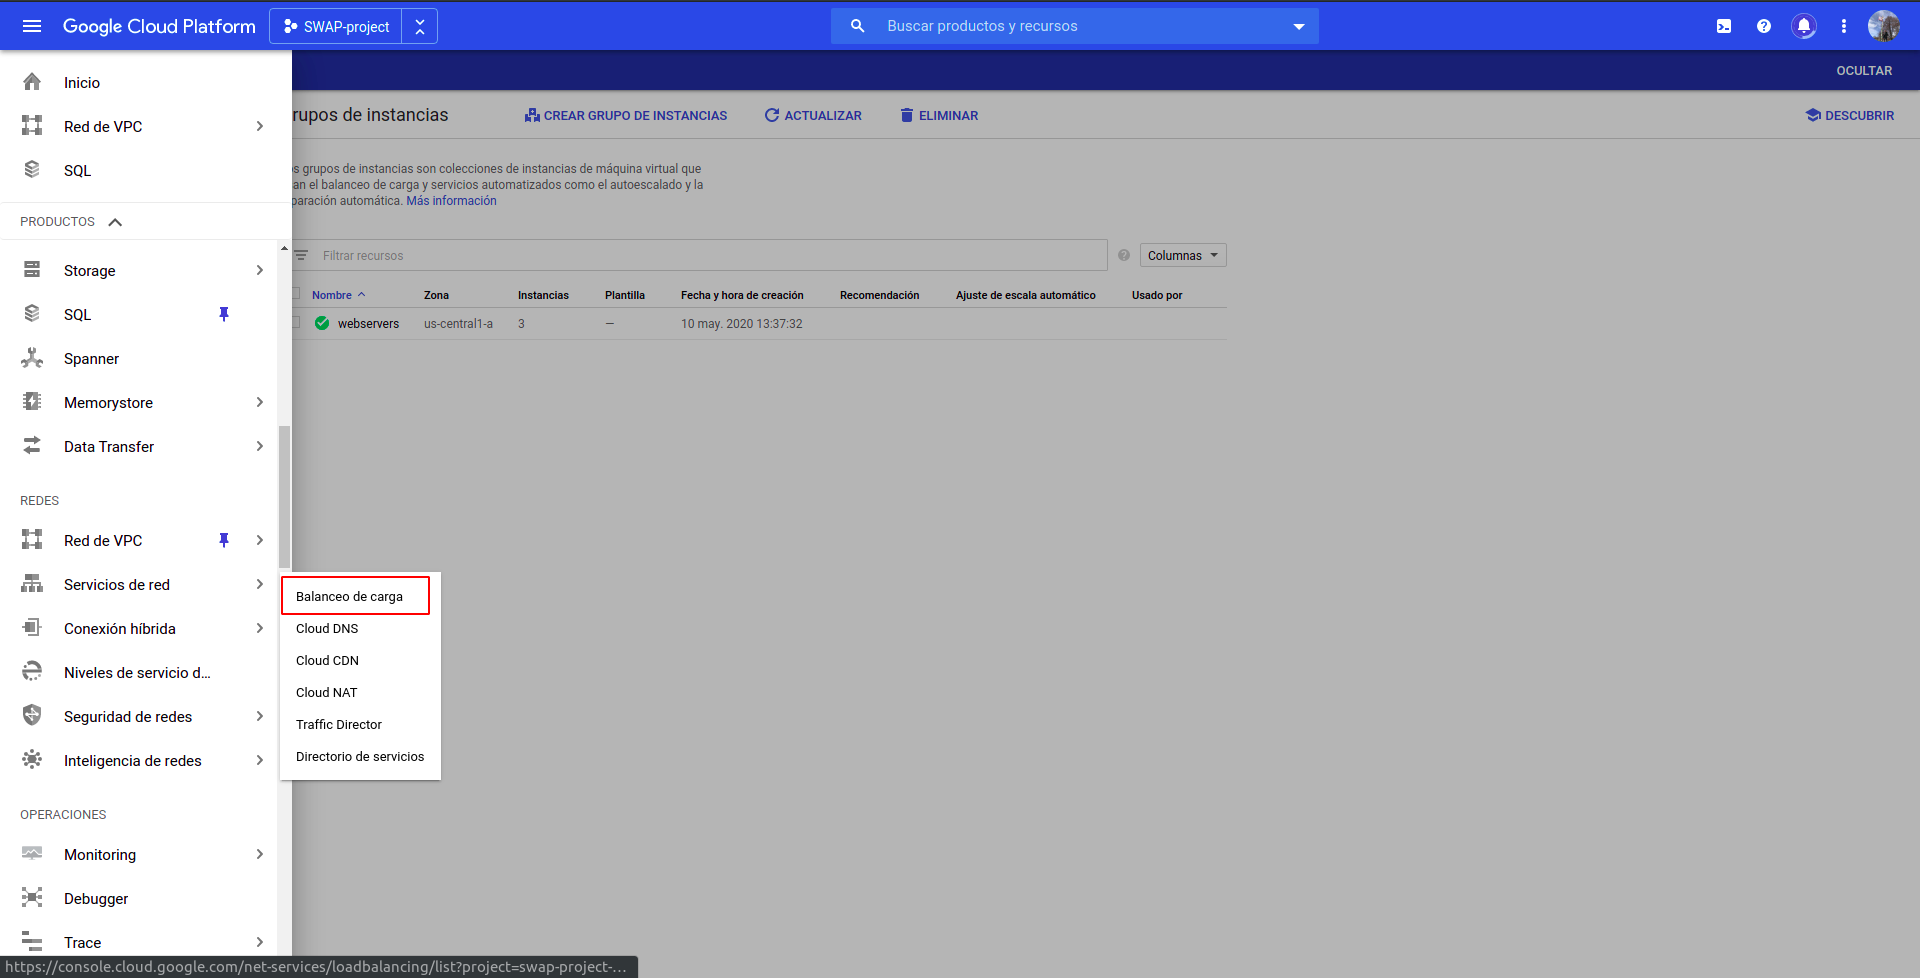
\includegraphics[width=\textwidth]{project/loadbalancer.png}
	\end{figure}
\end{frame}

\begin{frame}[fragile]{Creación del balanceador de carga HTTP(s)}
  \begin{figure}[H]
		\centering
		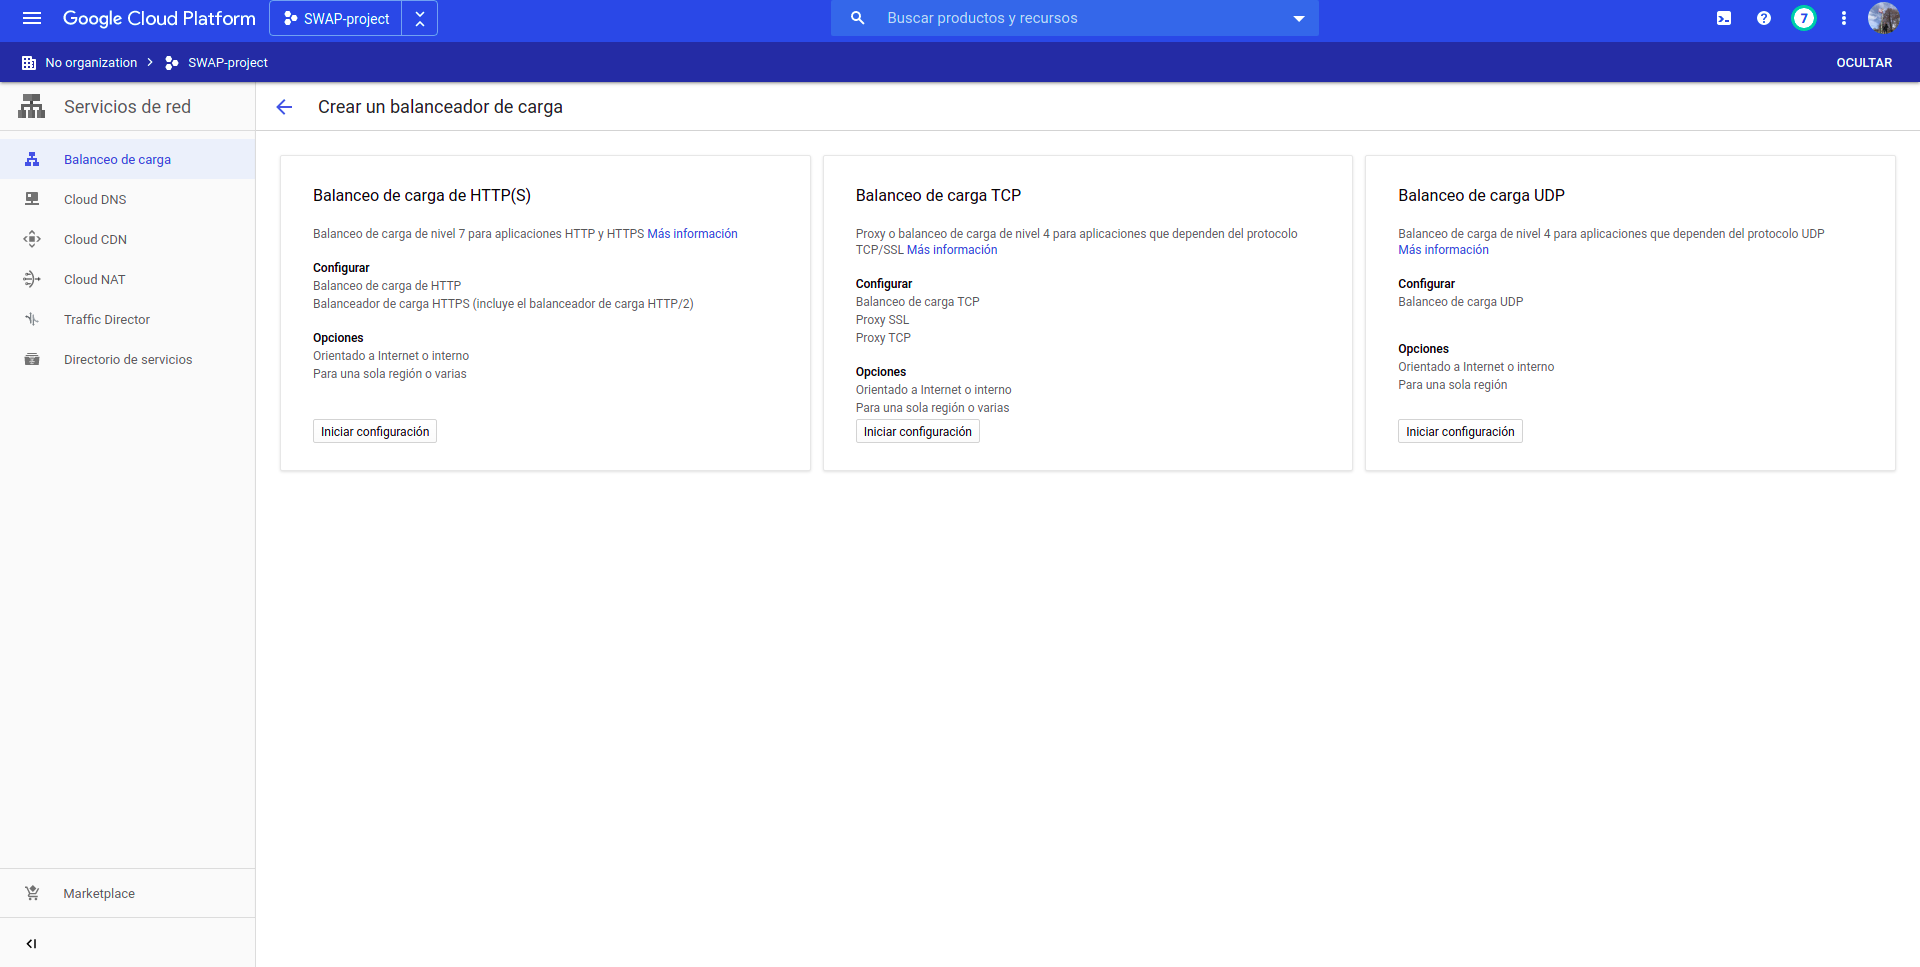
\includegraphics[width=\textwidth]{project/loadbalancerhttps.png}
	\end{figure}
\end{frame}

\begin{frame}[fragile]{Creación del balanceador de carga HTTP(s)}
  \begin{figure}[H]
		\centering
		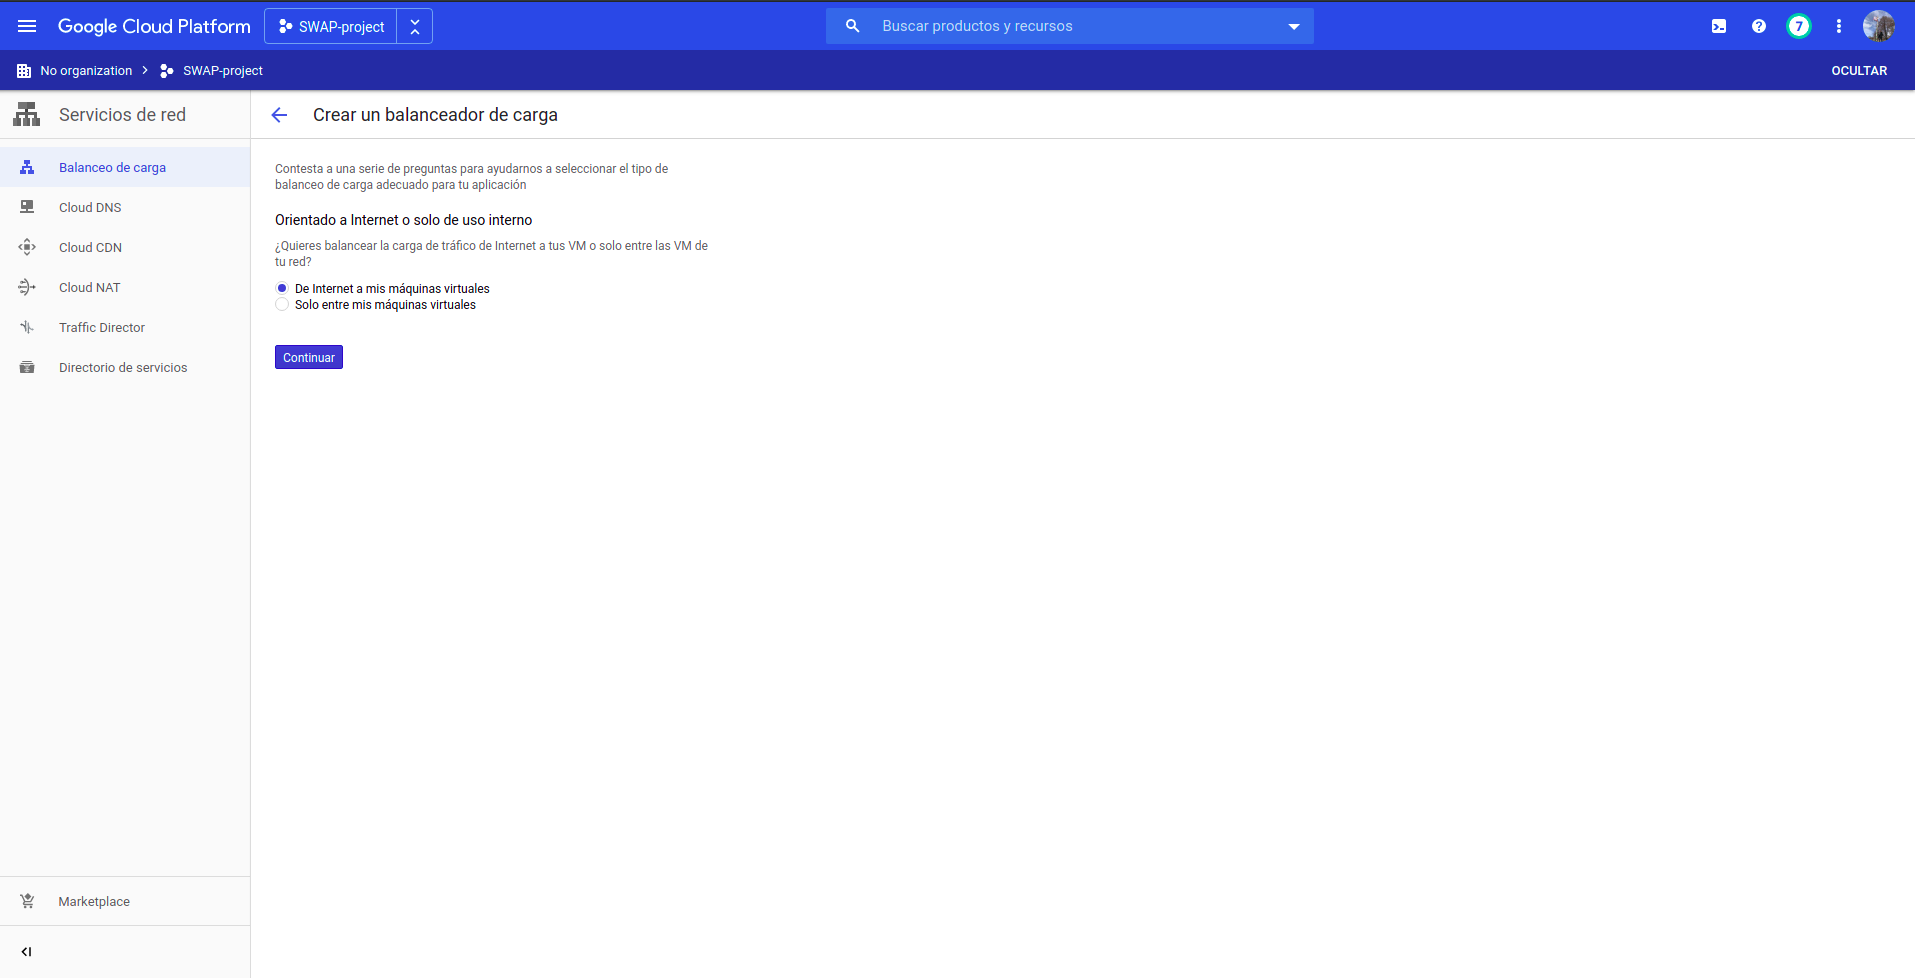
\includegraphics[width=0.65\textwidth]{project/frominternet.png}
	\end{figure}
\end{frame}

\begin{frame}[fragile]{Creación del backend}
  \begin{figure}[H]
		\centering
		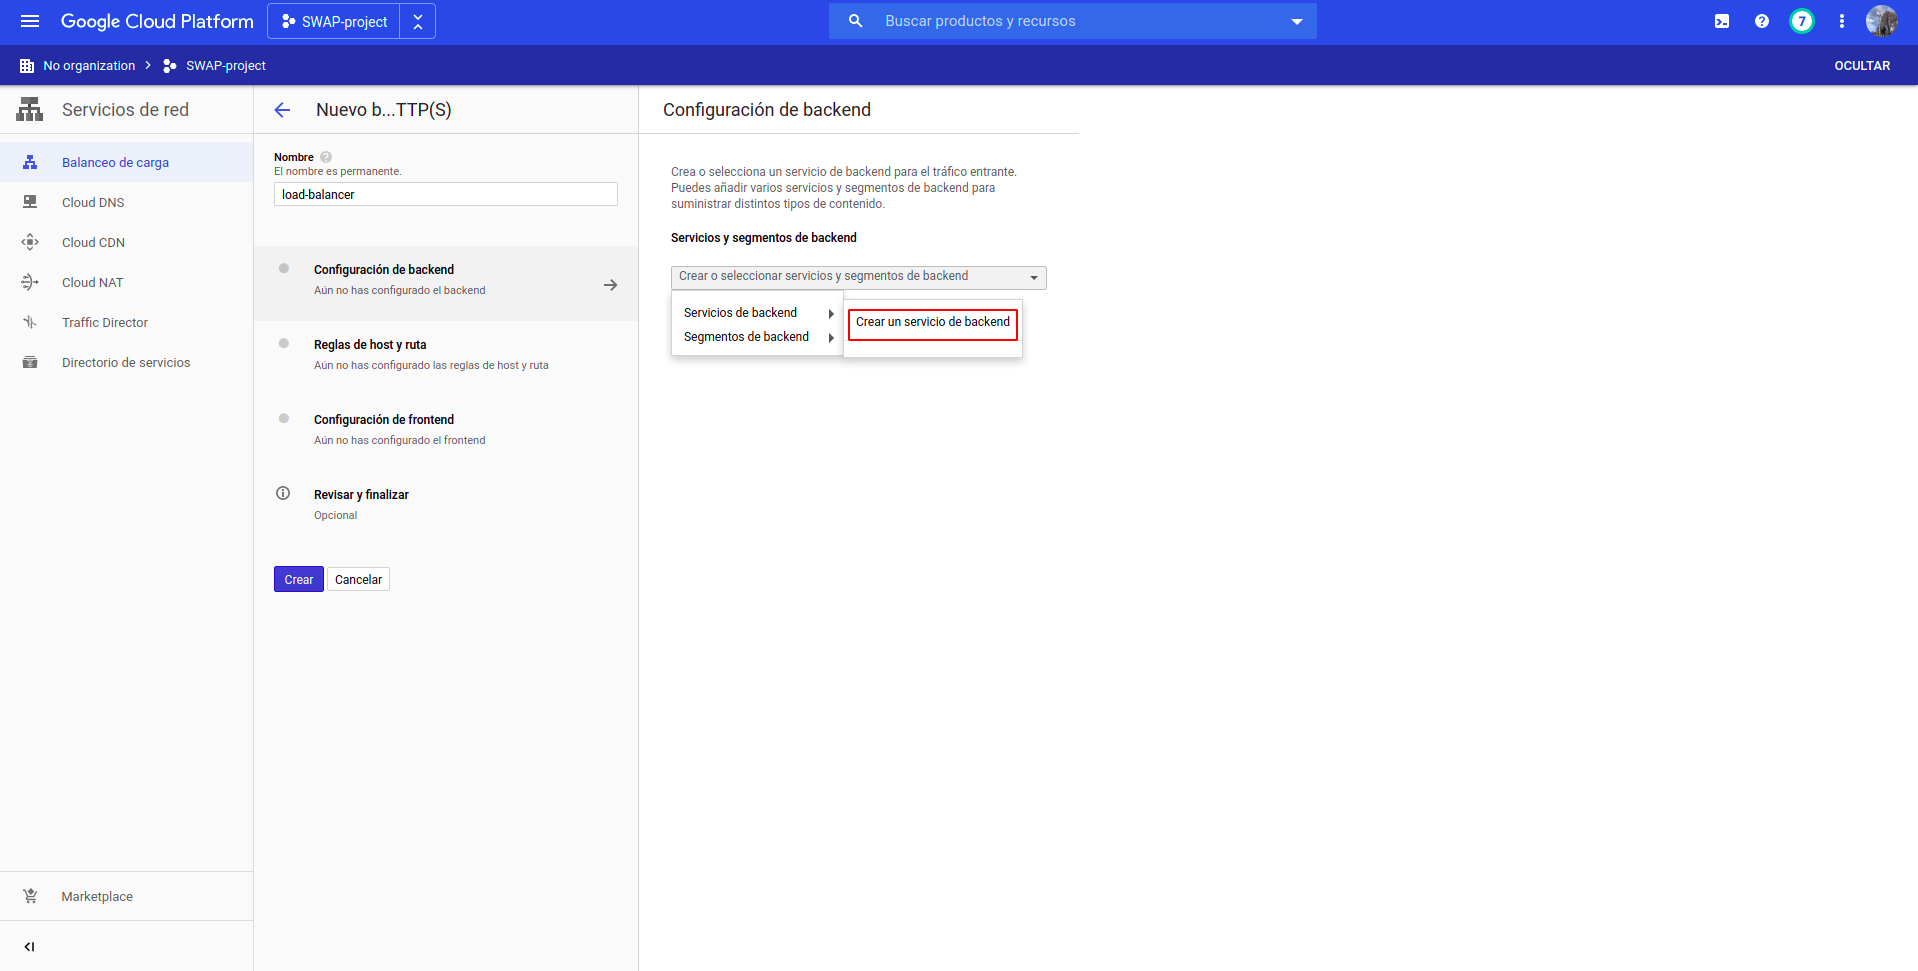
\includegraphics[width=0.65\textwidth]{project/backend.png}
	\end{figure}
\end{frame}

\begin{frame}[fragile]{Creación del backend - Selección de grupo de instancias}
  \begin{figure}[H]
		\centering
		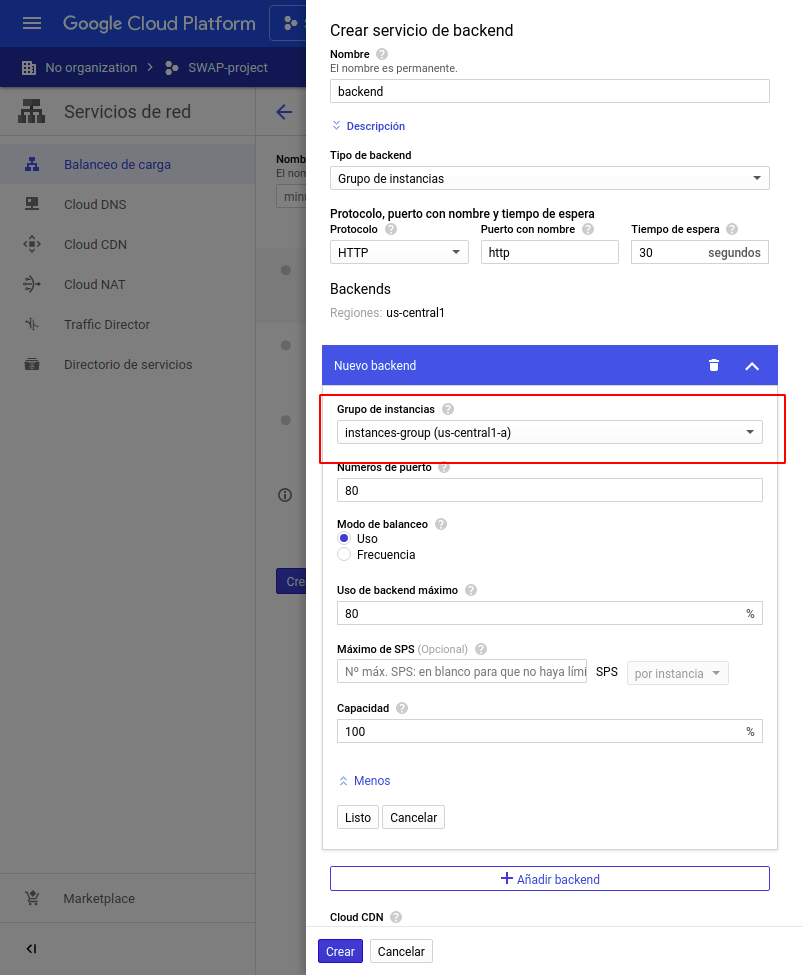
\includegraphics[width=0.65\textwidth]{project/backend_selection.png}
	\end{figure}
\end{frame}

\begin{frame}[fragile]{Creación de la comprobación de estado}
  \begin{figure}[H]
		\centering
		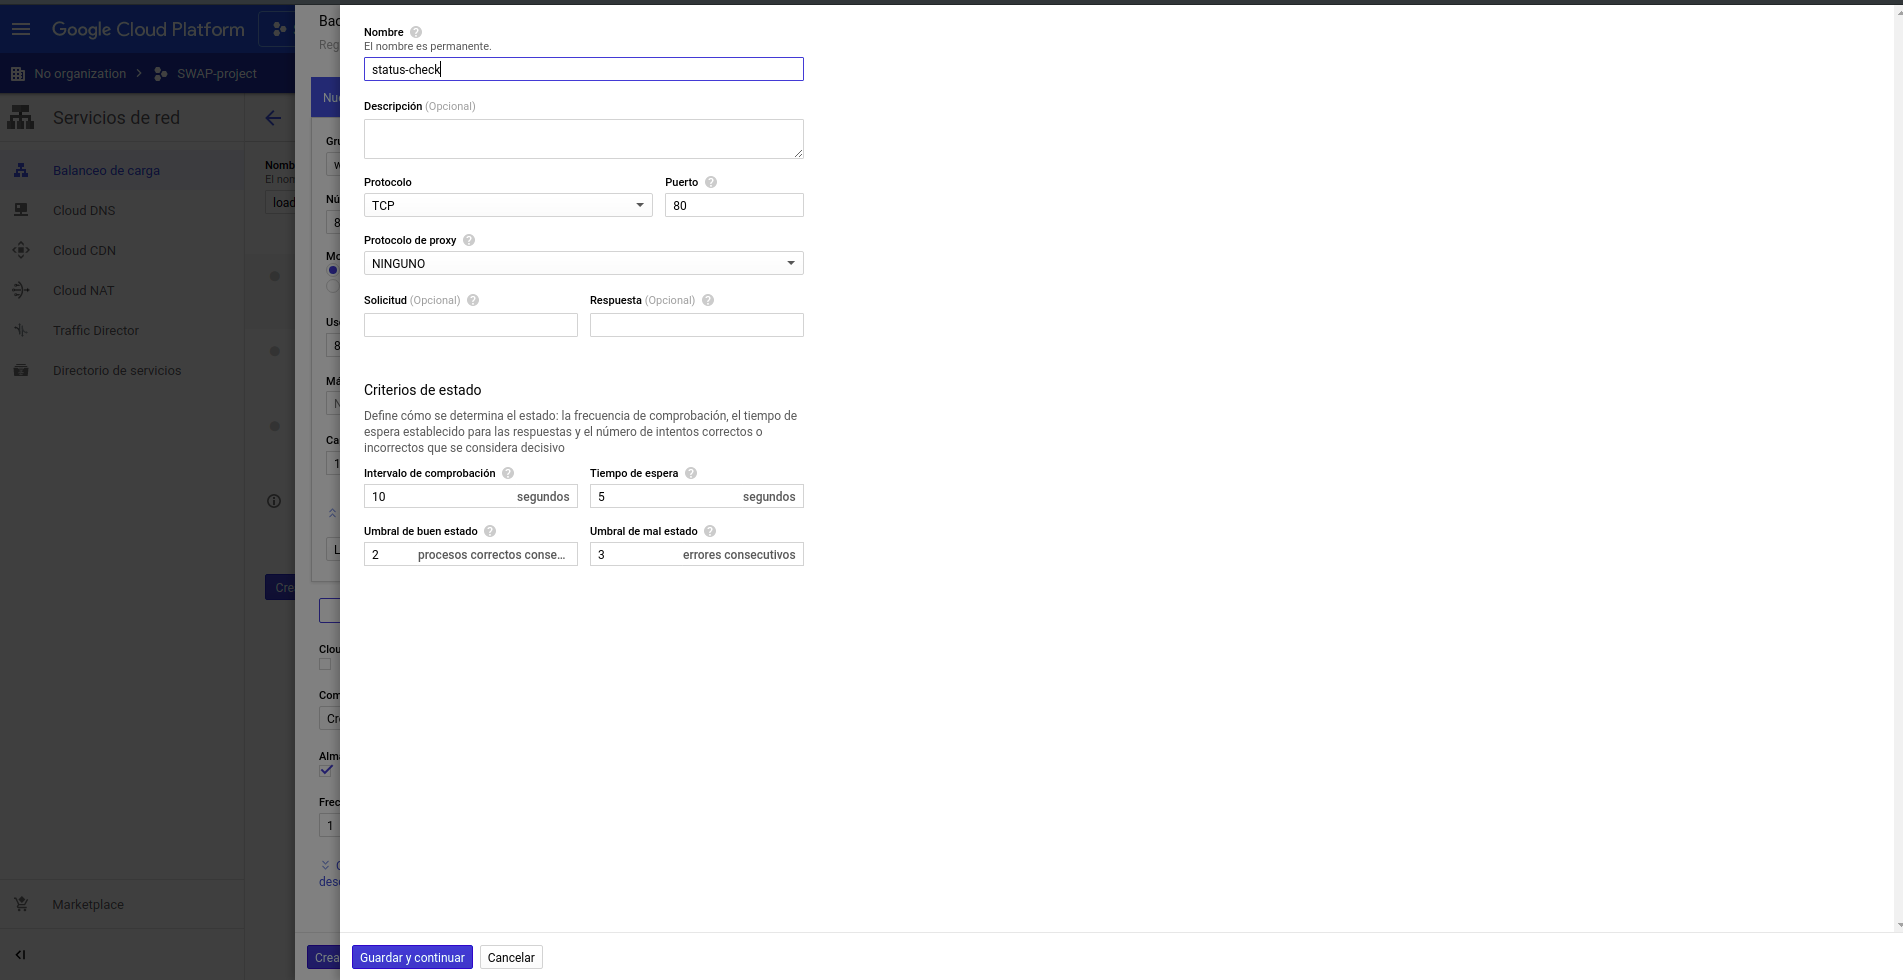
\includegraphics[width=0.35\textwidth]{project/status_check.png}
	\end{figure}
\end{frame}

\begin{frame}[fragile]{Creación del frontend}
  \begin{figure}[H]
		\centering
		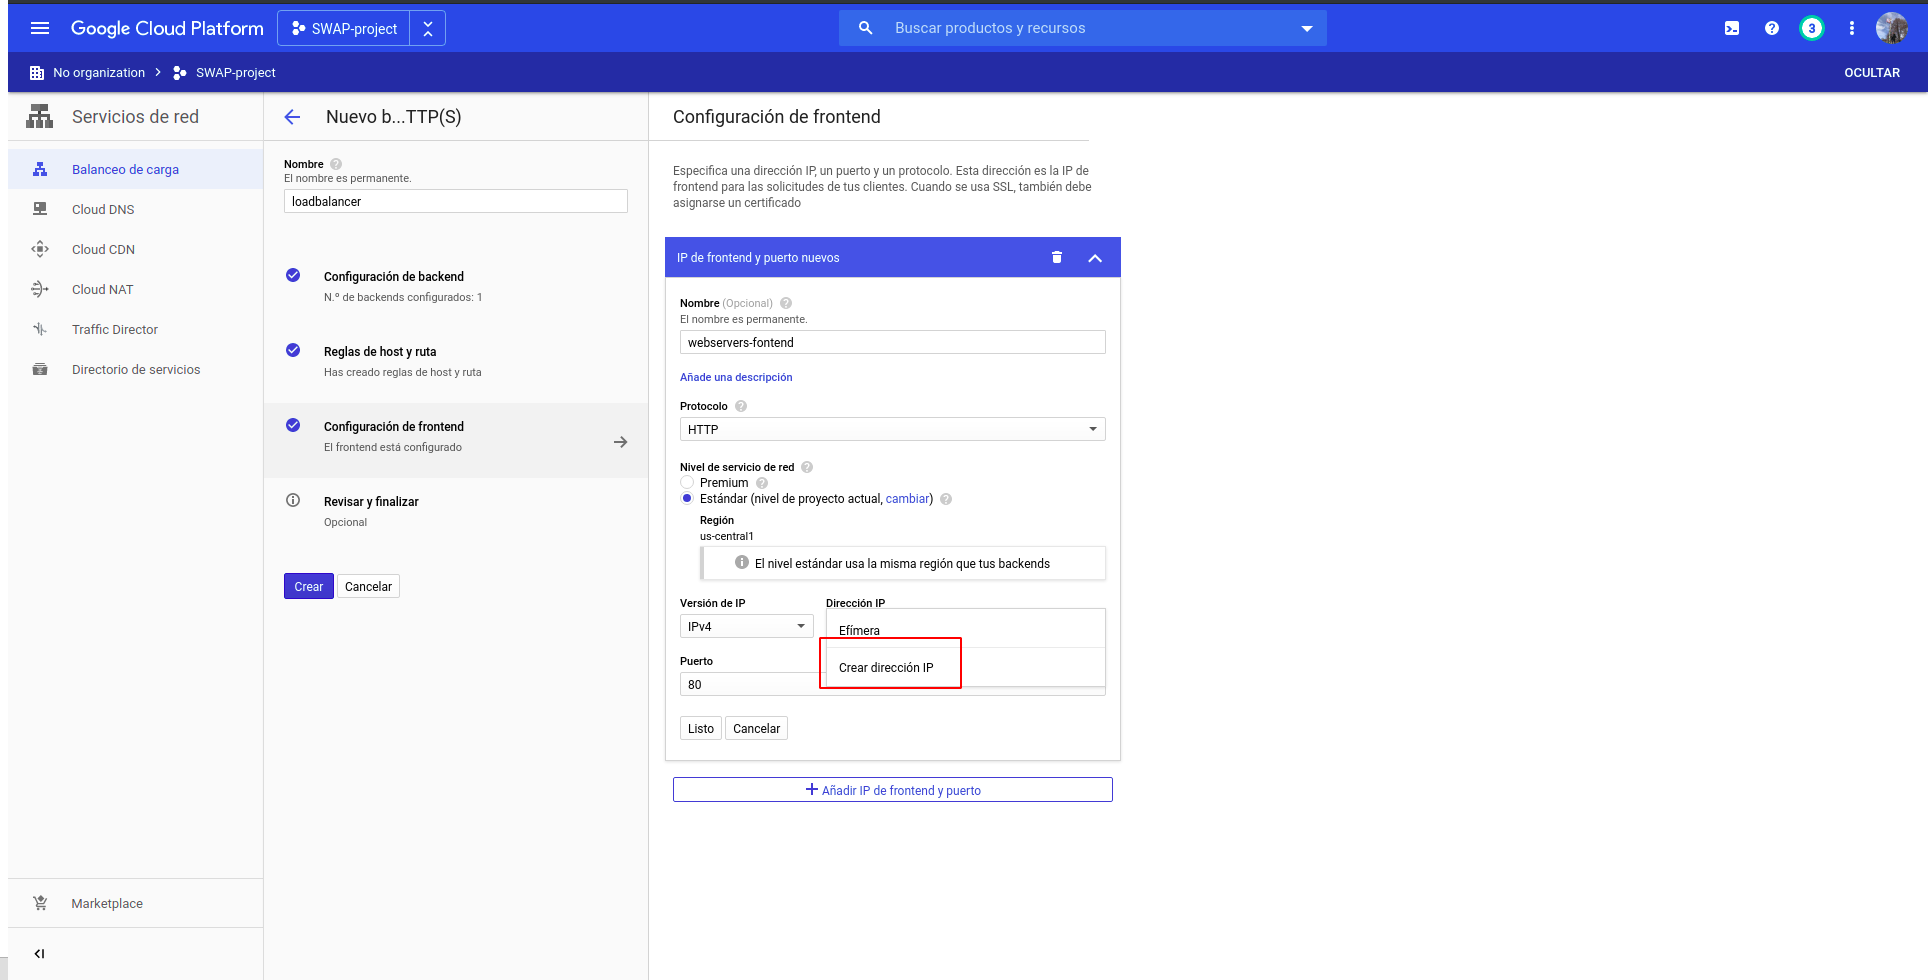
\includegraphics[width=0.8\textwidth]{project/frontend.png}
	\end{figure}
\end{frame}

\begin{frame}[fragile]{Comprobación de funcionamiento}
  \begin{figure}[H]
		\centering
		
\includegraphics[width=\textwidth]{project/load_balancer_ok.png}
	\end{figure}
\end{frame}

\subsection{Prueba de estrés}

\begin{frame}[fragile]{Test de estrés}
  \begin{figure}[H]
		\begin{lstlisting}
	host > ab -n 100000 -c 300
                http://35.208.234.230/
		\end{lstlisting}
\end{figure}
\begin{itemize}[<+->]
  \item 100000 peticiones
  \item 300 usuarios concurrentes
  \item IP del balanceador
\end{itemize}
\end{frame}

\begin{frame}[fragile]{Test de estrés - Resultados}
  \begin{figure}[H]
	    \centering
			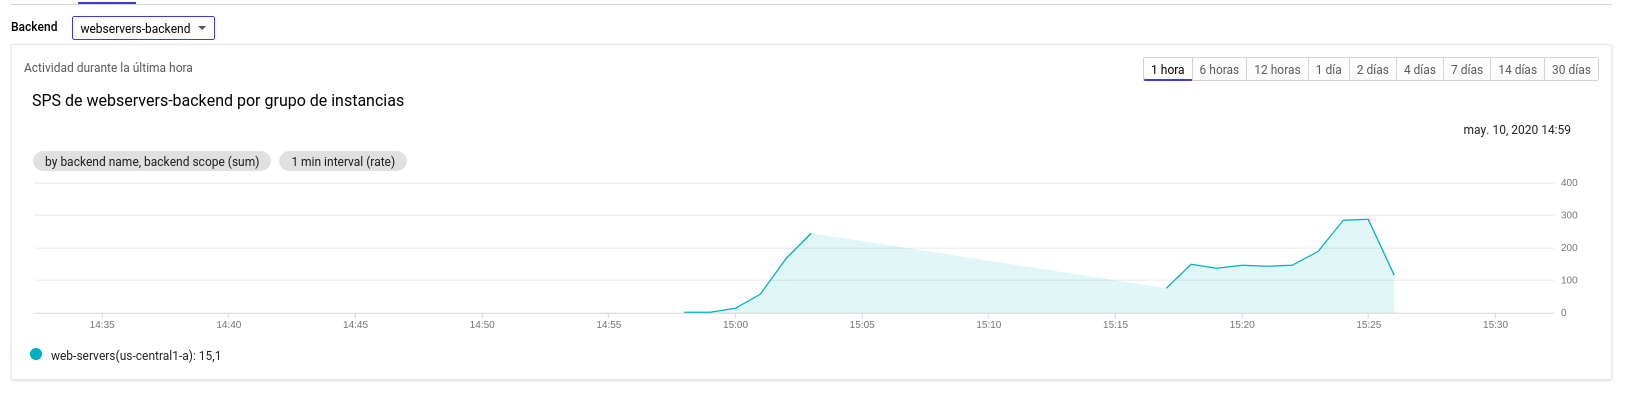
\includegraphics[width=\textwidth]{project/monitoring.png}
			\caption{Monitorización del balanceador de carga}
	\end{figure}
\end{frame}
\begin{frame}[fragile]{Test de estrés - Resultados}
  \begin{figure}[H]
	    \centering
			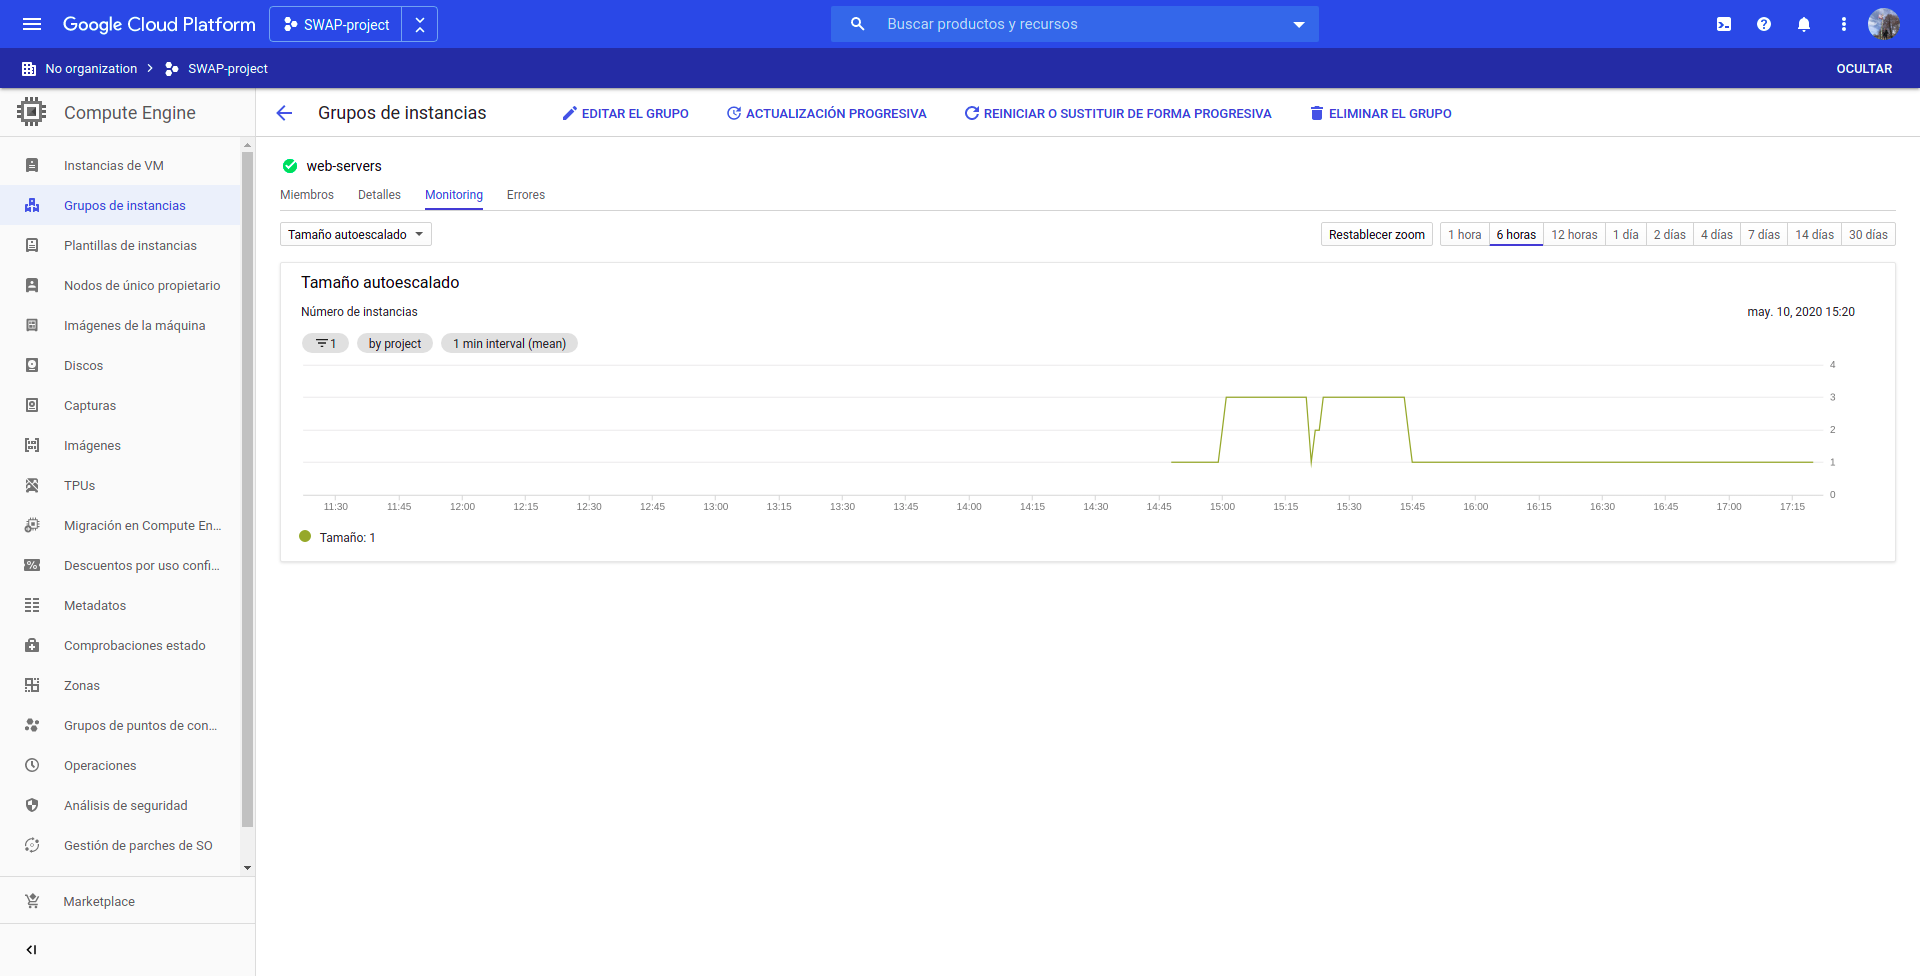
\includegraphics[width=\textwidth]{project/monitoring_groups.png}
			\caption{Monitorización del grupo de instancias}
	\end{figure}
\end{frame}

\subsection{Asegurar la granja web}

\begin{frame}[fragile]{Asegurar la granja web}
  \begin{figure}[H]
		\centering
		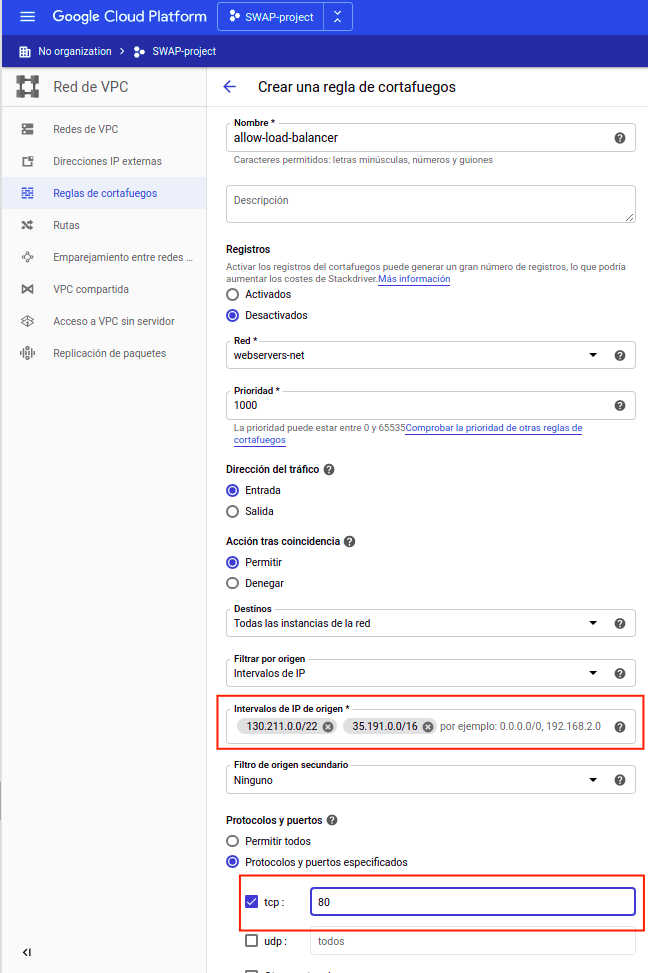
\includegraphics[width=0.45\textwidth]{project/firewall_balancer.png}
	\end{figure}
\end{frame}

\begin{frame}[fragile]{Asegurar la granja web - Comprobación}
  \begin{figure}[H]
		\centering
		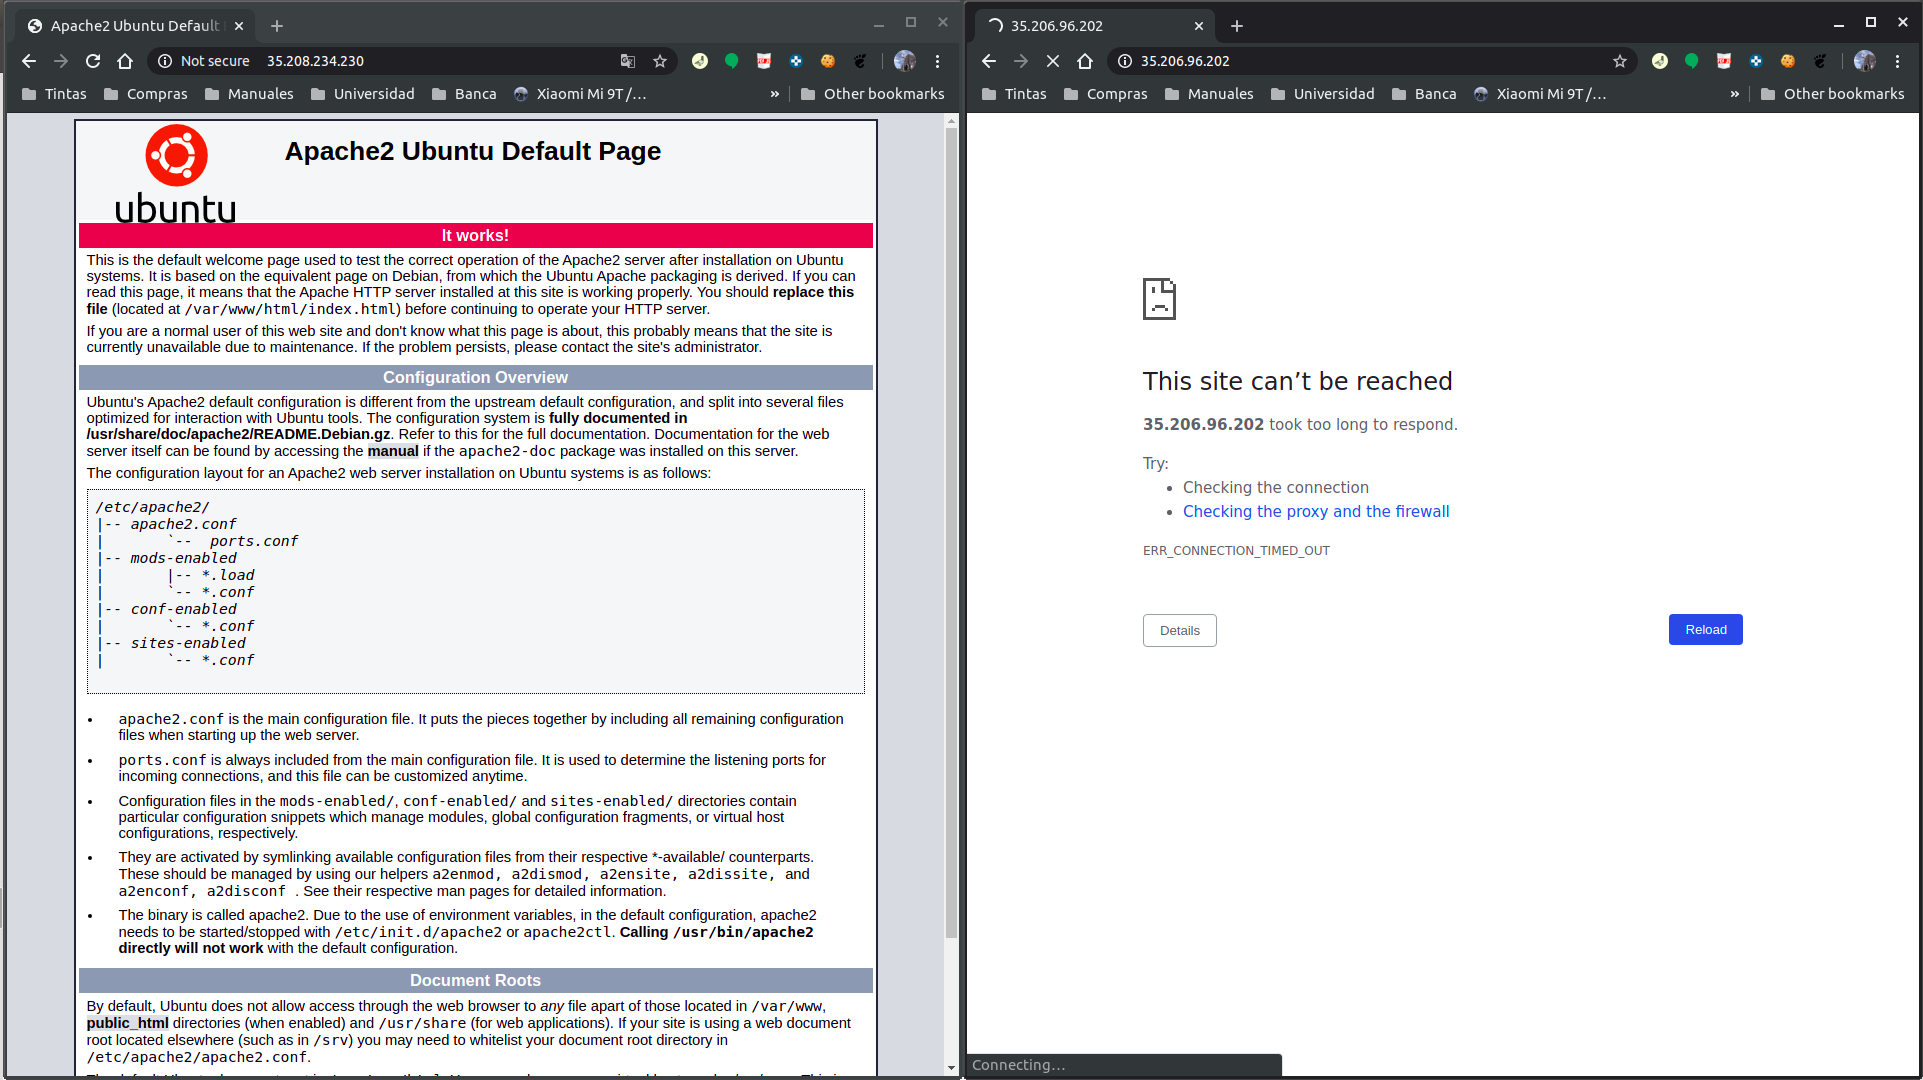
\includegraphics[width=\textwidth]{project/new_firewall_ok.png}
	\end{figure}
\end{frame}

\begin{frame}[fragile]
 \begin{center}
  \Huge
  Gracias por vuestra atención!
 \end{center}

\end{frame}

\end{document}
